% This is samplepaper.tex, a sample chapter demonstrating the
% LLNCS macro package for Springer Computer Science proceedings;
% Version 2.21 of 2022/01/12
%
\documentclass[runningheads]{llncs}
%
\usepackage[T1]{fontenc}
% T1 fonts will be used to generate the final print and online PDFs,
% so please use T1 fonts in your manuscript whenever possible.
% Other font encondings may result in incorrect characters.
%
\usepackage{graphicx}
% Used for displaying a sample figure. If possible, figure files should
% be included in EPS format.
%
% If you use the hyperref package, please uncomment the following two lines
% to display URLs in blue roman font according to Springer's eBook style:
%\usepackage{color}
%\renewcommand\UrlFont{\color{blue}\rmfamily}
%\urlstyle{rm}
%


%  Ed added the following packages %%%%%%%%%%%%%%%%%%%%%%%%%%
\usepackage{url}
%\def\UrlFont{\rmfamily}
\usepackage{graphicx}
\usepackage{amsmath}
\usepackage{epstopdf}% To incorporate .eps illustrations using PDFLaTeX, etc.
%\usepackage[caption=false]{subfig}% Support for small, `sub' figures and tables
%\usepackage[square,sort,comma,numbers]{natbib}

%\usepackage{fix-cm}
\usepackage{graphicx}  
\usepackage[hidelinks]{hyperref}  % for including hyperlinks in document, the hidelinks removes the green box in the pdf
%\usepackage{listings} % for source code listing
%\usepackage{color} % for source code listing

\usepackage{nccmath}
\usepackage{amssymb}% http://ctan.org/pkg/amssymb
%\usepackage{pifont}% http://ctan.org/pkg/pifont

%\usepackage{microtype} % relaxes the rules for inter word spacing 
%\usepackage[T1]{fontenc}
%\usepackage{lmodern}

\usepackage{tabularray}   % for table 
\usepackage{multirow}     % for centering content in a table 
%\usepackage{array, booktabs, ragged2e}
%\newcolumntype{P}[1]{>{\centering\arraybackslash}p{#1}}
%\newcolumntype{M}[1]{>{\centering\arraybackslash}m{#1}}

% Change the title of the Bibliography to References and make it left-justified
%\renewcommand{\bibname}{References}
%\makeatletter
%\renewcommand\bibsection{
	%	\section*{\refname\@mkboth{\MakeUppercase{\refname}}{\MakeUppercase{\refname}}}
	%}
%\makeatother

% Change the title of the Bibliography to References
%\def\bibname{References}

\usepackage{graphicx}
\usepackage[table,xcdraw]{xcolor}
% Beamer presentation requires \usepackage{colortbl} instead of \usepackage[table,xcdraw]{xcolor}

% Ed Stopped adding packages here %%%%%%%%%%%%%%%%%%

\begin{document}
%
\title{Title of your paper here}
%
% If the paper title is too long for the running head, you can set
% an abbreviated paper title here
\titlerunning{Your running title here ....}
%
%
\author{First Author\inst{1}\orcidID{0000-1111-2222-3333} \and
Second Author\inst{2,3}\orcidID{1111-2222-3333-4444} \and
Third Author\inst{3}\orcidID{2222--3333-4444-5555}}
%
% First names are abbreviated in the running head.
% If there are more than two authors, 'et al.' is used.
\authorrunning{F. Author et al. -- replace this with the authors}
%
%
\institute{Princeton University, Princeton NJ 08544, USA \and
Springer Heidelberg, Tiergartenstr. 17, 69121 Heidelberg, Germany
\email{lncs@springer.com}\\
\url{http://www.springer.com/gp/computer-science/lncs} \and
ABC Institute, Rupert-Karls-University Heidelberg, Heidelberg, Germany\\
\email{\{abc,lncs\}@uni-heidelberg.de}}
%
\maketitle              % typeset the header of the contribution
%
%
\begin{abstract}
The abstract should briefly summarize the contents of the paper in
150--250 words.

\keywords{First keyword  \and Second keyword \and Another keyword.}
\end{abstract}
%
%
\section{Introduction}
\label{Introduction}

This template is provided for the Research Project and Paper for the CIS*4150 Software Reliability and Testing course. It is based on the Springer Nature template, commonly used in academic journals and conferences. The template outlines how to structure your paper, include figures and tables, and cite references from the bibliography.

Once you have reviewed this document, replace the placeholder content with your own in the appropriate sections.

I hope you find this helpful!

Ed

The Introduction sets the stage for the research by providing a high-level overview of background information, defining the problem or research question, and explaining the study's objectives. It typically includes a couple key relevant papers to highlight gaps in current knowledge, justifies the need for the study, and outlines the paper's structure. The introduction should engage the reader by clearly explaining why the research is important and what the study aims to contribute to the field. It often ends with a brief summary of the research approach or hypothesis.


Generative AI, encompassing technologies such as Large Language Models (LLMs) like ChatGPT, and advanced image generation tools, is profoundly reshaping various facets of the digital and real world. As educators and researchers, it is essential to stay abreast of these advancements to enhance our teaching methods and pedagogical tools, thereby enriching both our own and our students' skillsets.

This research delves into the specific application of LLMs, focusing on ChatGPT, to assess its impact on developing academic critique skills among Computer Science undergraduates enrolled in a fourth-year Ubiquitous Computing course. The core objective of this study is to evaluate and discern the differences between student-authored critiques and those augmented by ChatGPT's assistance.

Through this investigation, we aim to highlight the potential of LLMs to bolster students' critical thinking and writing capabilities. This paper seeks to provide valuable insights into how AI tools can be seamlessly integrated within educational frameworks.  Additionally, we explore the transformative role of AI-driven tools in supporting student learning and enhancing the personalized and engaging nature of academic critique processes.

The remainder of this paper is structured as follows: The next section offers a background on Generative AI, focusing on the Transformer architecture, ChatGPT, its applications in education, and readability metrics. In Section~\ref{Methodology}, we outline the methods employed to investigate the effectiveness of ChatGPT as a collaborative tool for supporting technical critique writing. The findings from our quantitative and qualitative analysis are presented in Section~\ref{Findings}. Section~\ref{Discussion} reflects on these findings within a broader context, and Section~\ref{Conclusion} concludes the paper while highlighting potential future directions for this line of research.
\section{Background}
\label{Background}

Replace all this with a relevant comprehensive literaure review in your specific area of interest in Software Testing.  The Background section provides context and detailed information needed to understand the research problem. It typically includes a review of existing literature, key concepts, theories, and previous studies relevant to the topic. The goal is to frame the research by outlining what is already known, identifying gaps in the knowledge, and explaining why the current study is necessary. The background helps the reader understand how the research fits into the broader field and what it aims to contribute. 

The rapid evolution of Generative AI has profoundly transformed technological capabilities, significantly influencing societal interactions, business processes, and educational methodologies. This section is divided into three main parts. The first part delves into the key technologies that have driven this transformation, highlighting their impact and implications. The second part presents an overview of current applications of Generative AI in the context of education, exploring how these innovations are being integrated into teaching and learning environments. The last section presents an overview of various readability metrics commonly used in the assessment of text.

\subsection{Foundations of Generative AI}
Before 2017, Natural Language Processing (NLP) relied heavily on architectures like Constitutional Neural Networks, Recurrent Neural Networks (RNNs), Gated Recurrent Units (GRUs), and Long Short-Term Memory networks (LSTMs)~\cite{sherstinsky_2020_fundamentals}. These architectures were adept at processing sequences and were widely used for various NLP tasks. However, they often struggled with long-range dependencies and were computationally intensive due to their sequential nature, limiting their scalability and performance on larger datasets~\cite{sherstinsky_2020_fundamentals}.

NLP took a major leap forward in 2017 with the introduction of the \textit{Transformer} model by Vaswani et al.~\cite{vaswani2017_Attention}. It marked a paradigm shift in sequence modeling, emphasizing the importance of self-attention mechanisms~\cite{vaswani2017_Attention}. Essential for developing models that require a complex understanding of sequence data, such as those used in real-time language translation and interactive conversational agents, the Transformer architecture has become a core component of many state-of-the-art AI systems, influencing advancements across numerous fields including healthcare, finance, and autonomous vehicles.

\begin{figure}
	\centering
	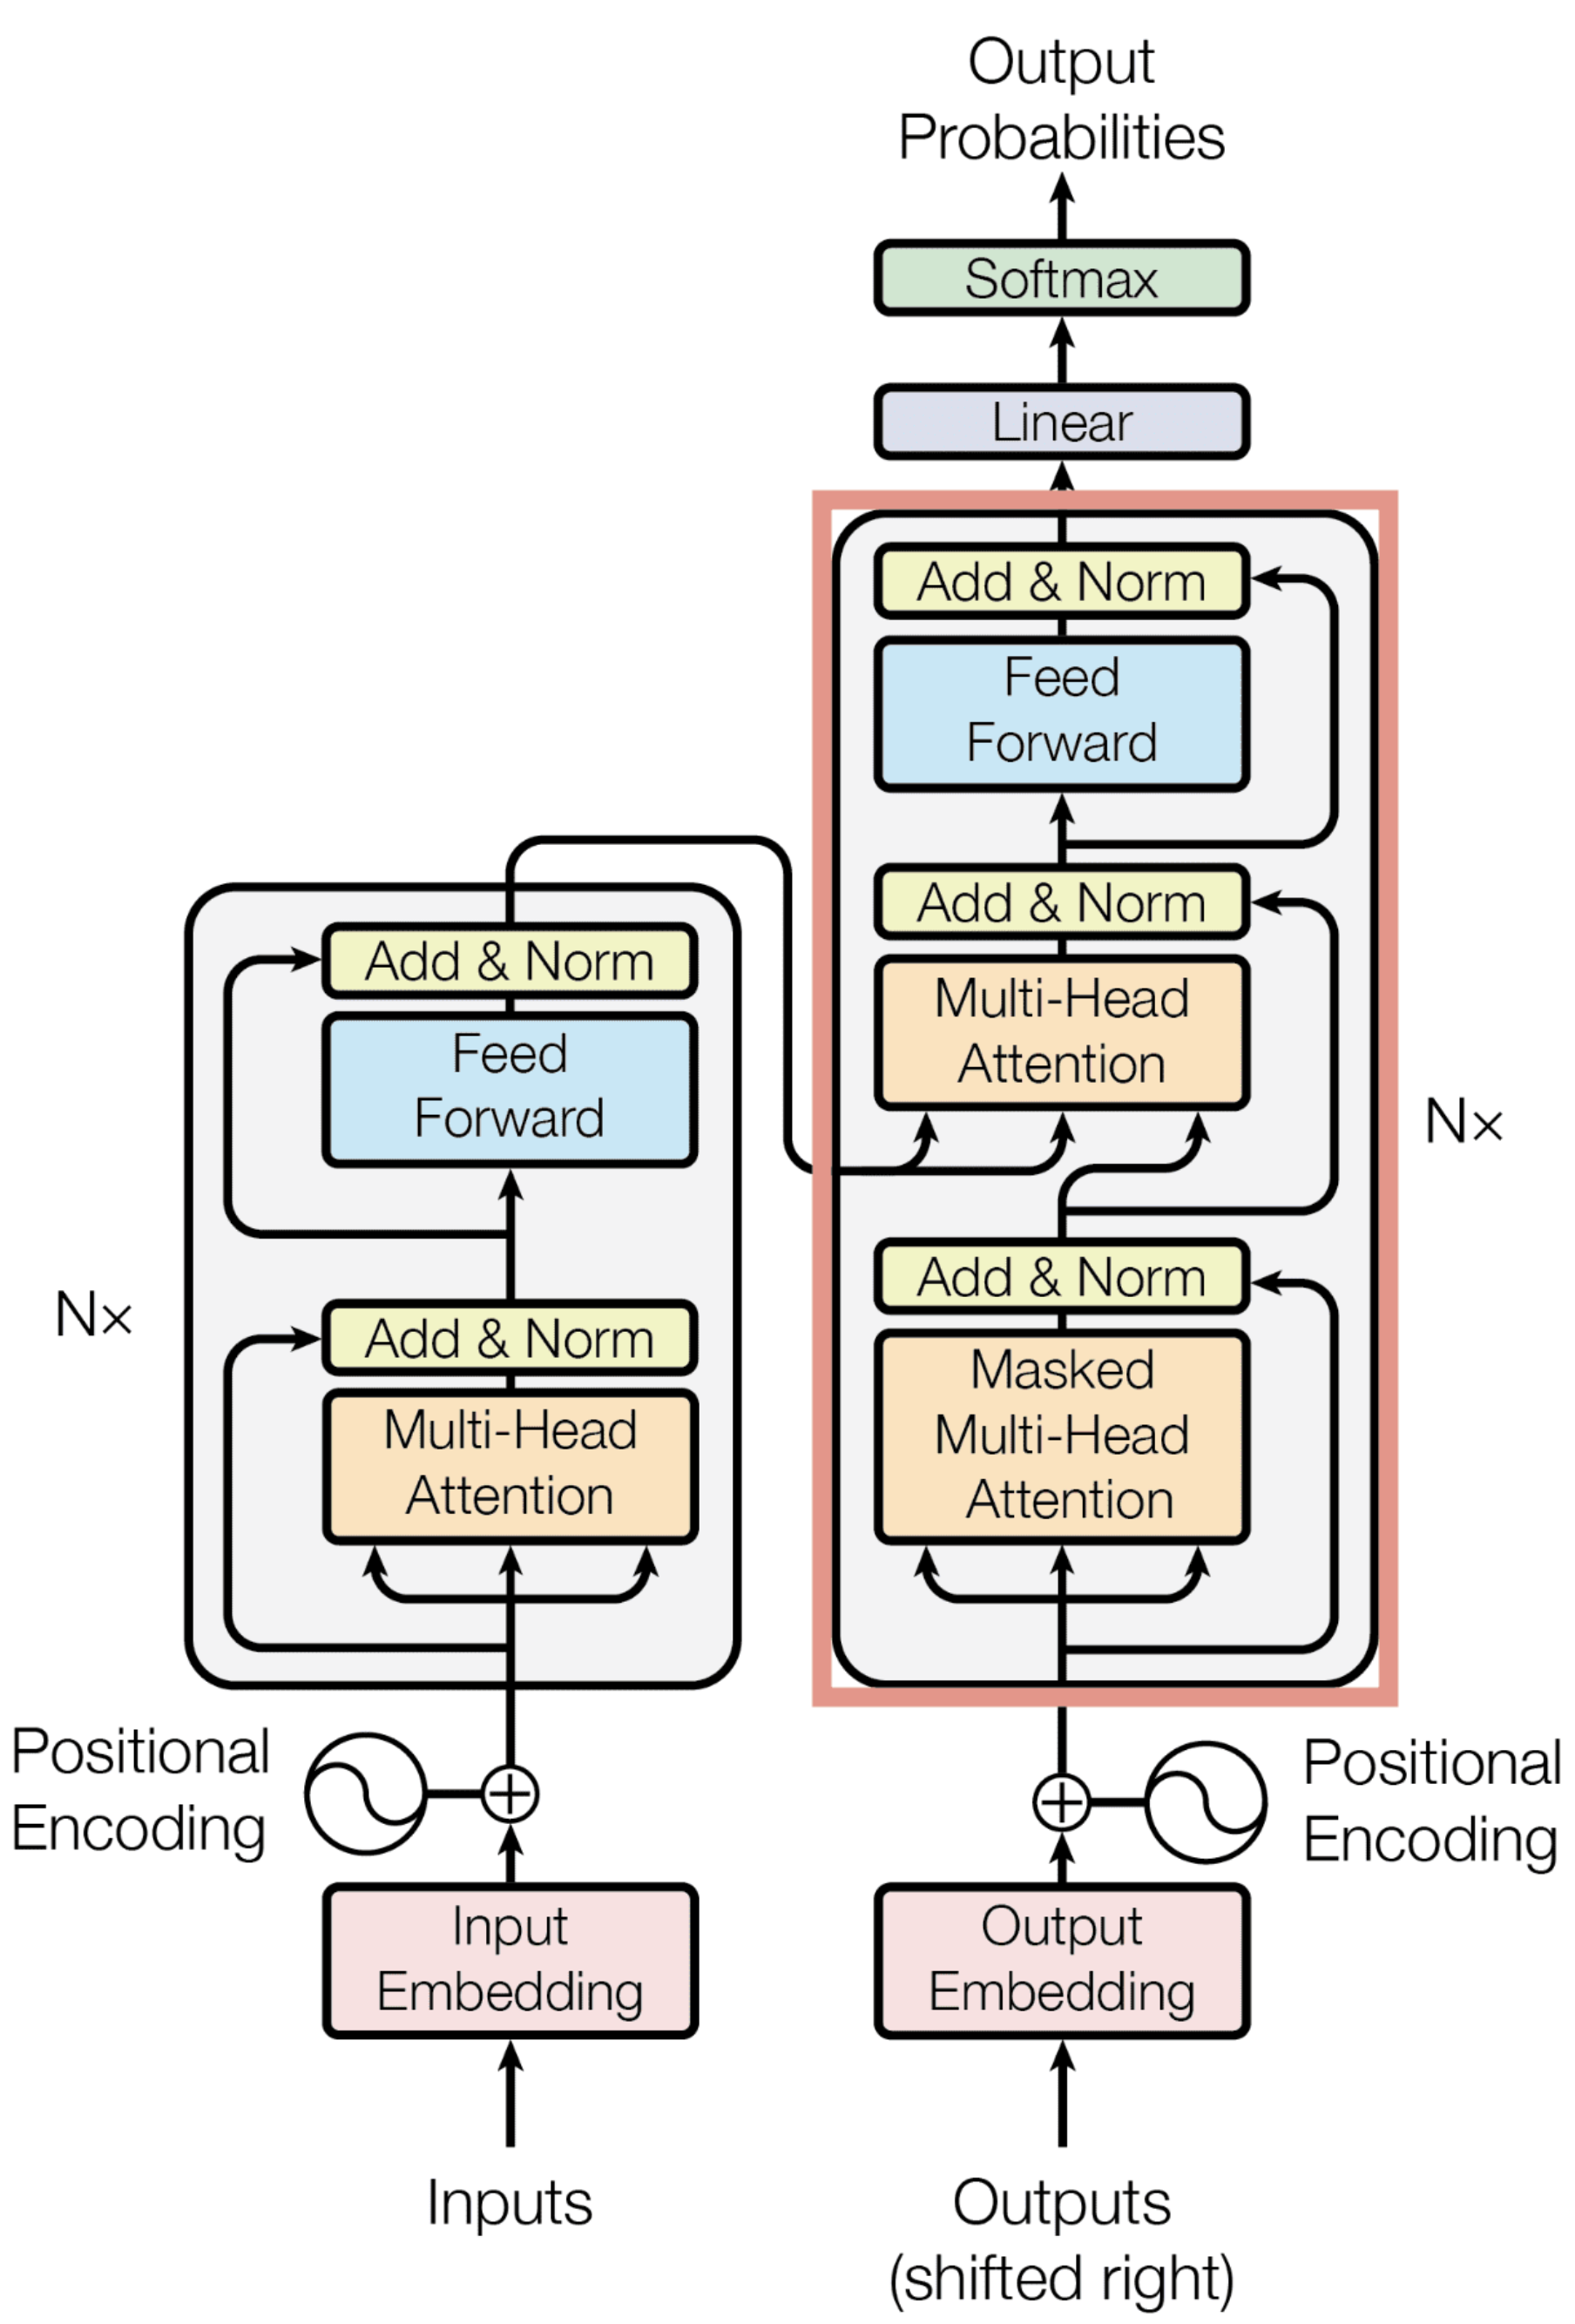
\includegraphics[width=0.8\linewidth]{figures/transformer_architecture}
	\caption[Transformer Architecture]{The Transformer -- model architecture~\cite{vaswani2017_Attention}}
	\label{fig:Transformer_Architecture}
\end{figure}

Following the Transformer's success, Google AI's BERT (Bidirectional Encoder Representations from Transformers) emerged as a significant advancement, leveraging the Transformer's architecture to enhance language understanding~\cite{devlin2018_BERT}. BERT revolutionized natural language understanding by employing a transformer-based mechanism that processes words in the context of the entire sentence, rather than in isolation~\cite{devlin2018_BERT}. This breakthrough has led to substantial improvements in a range of language processing tasks, including translation, text summarization, and sentiment analysis. BERT's architecture leverages a stack of transformer blocks that feature two key components: multi-head self-attention mechanisms and fully connected feed-forward networks. This architecture enables the model to capture complex word relationships and contextual nuances across different parts of the text, facilitating more effective learning and prediction capabilities compared to previous models. BERT is also trained on a large corpus of text in a self-supervised manner using two tasks: masked language modeling and next sentence prediction, which help improve its language understanding. Figure~\ref{fig:BERT_architecture} presents the BERT architectural model, illustrating its deep neural network structure and attention mechanisms that contribute to its powerful performance.

\begin{figure}
	\centering
	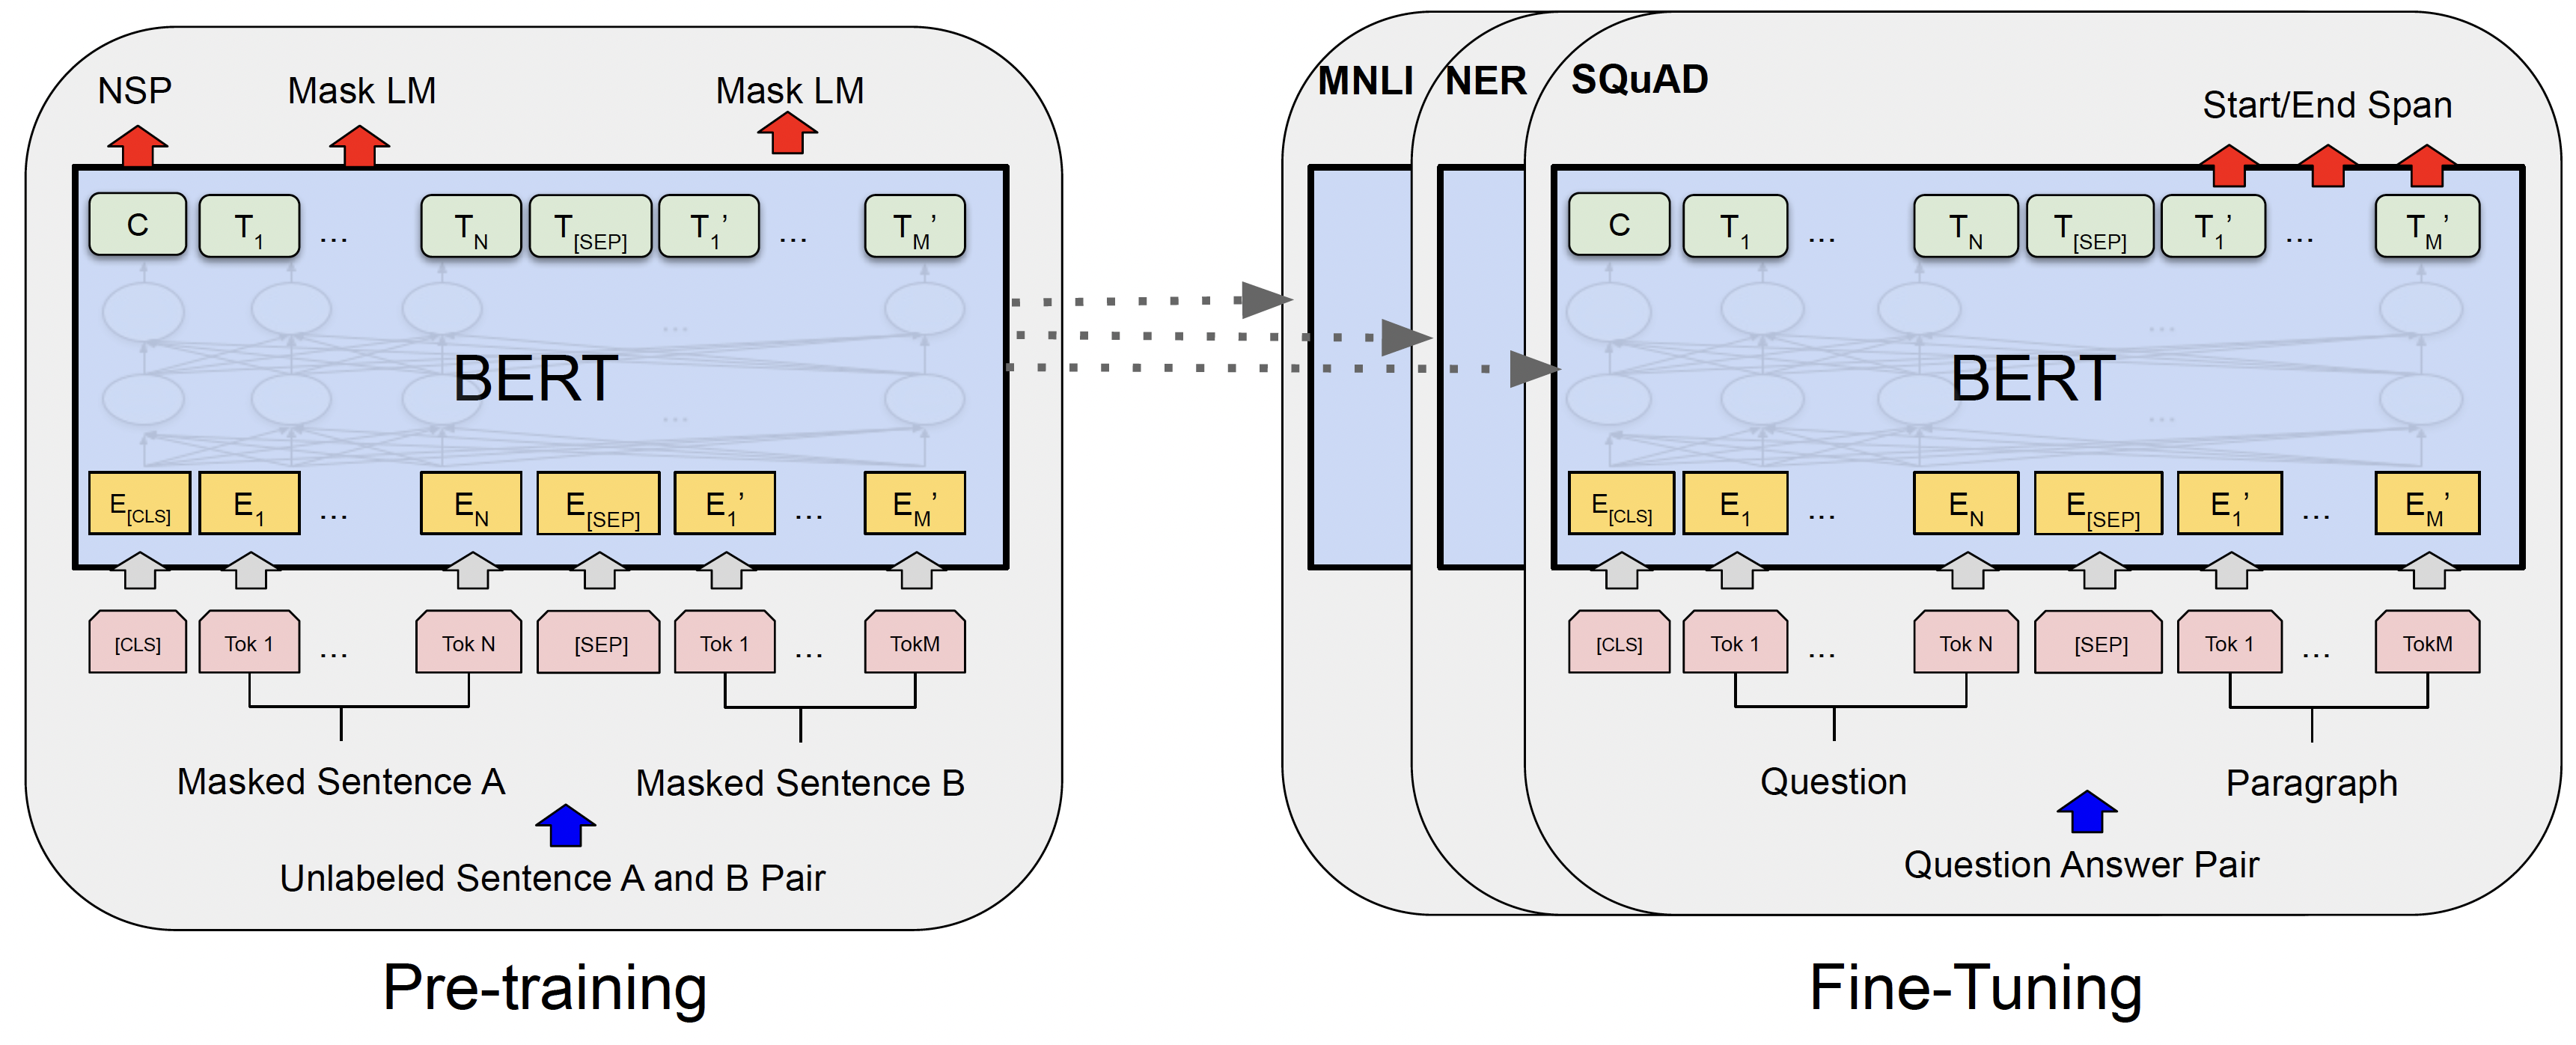
\includegraphics[width=1.0\linewidth]{figures/BERT_Architecture}
	\caption[BERT architectural model]{BERT architectural model~\cite{devlin2018_BERT}}
	\label{fig:BERT_architecture}
\end{figure}

Building on BERT’s architecture, RoBERTa (Robustly Optimized BERT Approach) by Facebook AI modified key training methodologies to optimize performance~\cite{liu2019_RoBERTa}. Specifically, RoBERTa is trained with dynamic masking, full-sentences without NSPloss, large mini-batches, and a larger byte-level BPE~\cite{liu2019_RoBERTa}. Additionally, RoBERTa includes two other important components that were under-emphasized in the BERT architecture, namely: (1)~the data used for pretraining, and (2)~the number of training passes through the data. The RoBERTa model is trained on more data, with larger batches and longer sequences. As a result, RoBERTa offers a significant improvement in its language understanding capabilities, pushing the boundaries of what AI can comprehend and respond to, thereby setting new standards for model robustness and accuracy in language tasks~\cite{liu2019_RoBERTa}.

Since 2019, Hugging Face has emerged as a pivotal player in democratizing AI through the development and maintenance of the Transformers library, which provides a vast collection of pre-trained models for a variety of NLP tasks~\cite{wolf2020transformers}. This open-source library has enabled researchers and practitioners to easily implement cutting-edge models, fostering innovation and accelerating the adoption of AI technologies across industries. Currently, there are over 200 different transformer models available from Hugging Face: \url{https://huggingface.co/docs/transformers/index}.

The Generative Pre-trained Transformer (GPT) series, developed by OpenAI, includes notable releases such as GPT-2 in 2019, GPT-3.5 in 2022, and GPT-4 in 2023. Each iteration has progressively expanded the scale and capabilities of language models~\cite{radford2019_language,brown2020_language}. With each version, there has been a significant leap in sophistication; for instance, GPT-4 is capable of producing text that closely mimics human writing across a wide range of genres and styles. These advancements underscore the creative potential of AI in generating coherent and contextually relevant text. However, they also bring to light critical ethical considerations, including concerns over misinformation, copyright issues, and the autonomy of AI-driven content creation. 

Figure~\ref{fig:GPT_Architecture} presents the architecture of the Generative Pre-trained Transformer. The GPT architecture is built upon the foundation of the Transformer model, which utilizes layers of self-attention mechanisms to process text~\cite{wolf2020transformers}. At the core of the GPT architecture, as illustrated in the figure, is a series of Transformer blocks stacked on top of each other. Each block contains two main sub-layers: a \textit{multi-head self-attention} mechanism and a \textit{position-wise fully connected feed-forward network}.

Input embeddings, which convert tokens (words or pieces of words) into vectors of numbers, are first modified by positional encodings to retain the sequence order of the input text. These embeddings then pass through the Transformer blocks, where the self-attention mechanism allows the model to weigh the importance of different words relative to each other, regardless of their position in the text. This is followed by normalization and feed-forward layers that help in refining the representation with nonlinear transformations.

Each attention head in the multi-head attention layer computes an \textit{attention score}, which represents how much focus to place on other parts of the input sentence as each word is processed. The attention outputs are then combined and linearly transformed into the expected dimensions. Dropout layers are incorporated to prevent overfitting by randomly omitting subsets of features during training. The entire process within a Transformer block is designed to be differentiable so that it can be efficiently trained using gradient descent-based optimization.

This architecture enables GPT to generate text by predicting the next word in a sentence based on the words that came before it, learning to generate coherent and contextually relevant language over time. This capability makes GPT highly effective for a range of applications from automated content generation to sophisticated conversation simulations.

\begin{figure}
	\centering
	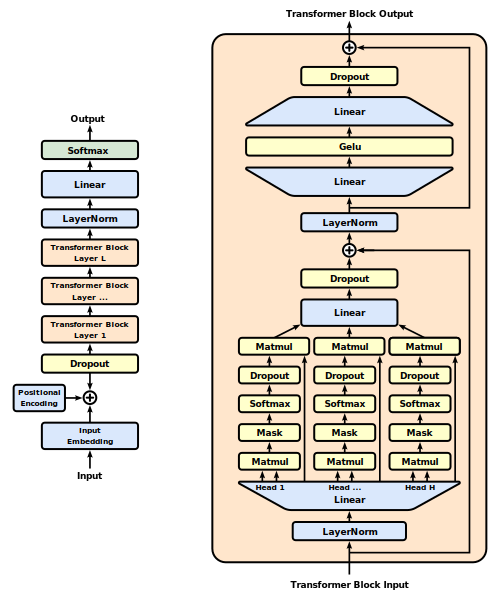
\includegraphics[width=1.0\linewidth]{figures/Full_GPT_architecture}
	\caption[Transformer Architecture]{The GPT Architecture~\cite{brown2020_language}}
	\label{fig:GPT_Architecture}
\end{figure}

In 2020 Facebook AI Research published a paper on Retrieval-Augmented Generation (RAG) which introduces an approach that combines the generative capabilities of models like GPT with the retrieval of factual information during the generation process~\cite{lewis2020retrieval}. This methodology enhances the model's ability to produce relevant and accurate responses by dynamically retrieving context from a vast corpus of data, representing a significant advancement in efforts to bridge the gap between human-like understanding and AI output.  Some examples of RAG models include:
\begin{enumerate}
	\item \textit{Call centre agent support}. Call centre agents require extensive knowledge of potentially hundreds of products and services, as well as commonly occurring product issues and their resolution. RAG solutions could assist agents in quickly finding answers to client requests.
	\item \textit{Customer chatbots}. RAG is strong enabler for creating customer-facing chatbots to answer frequently asked questions. Combining the natural language abilities of LLMs and the enterprise-specific responses of RAG can deliver a compelling, conversational customer experience.  
	\item \textit{Support / helpdesk}. Similar to call centre agents, IT operations and support personnel require deep knowledge of the configuration of complex systems deployments along with knowledge of common and previously seen issues and their resolution. RAG solutions could assist support personnel with quickly finding relevant answers to reported problems and observed issues.
\end{enumerate}

In the context of education, RAG offers transformative potential for educational environments by enhancing personalization, efficiency, and interaction in learning processes. By combining the generative capabilities of models like GPT with dynamic information retrieval, RAG can create tailored educational content, support research and writing, and enhance interactive tutoring systems~\cite{lewis2020retrieval}.  RAG's ability to pull relevant data from extensive knowledge bases allows it to generate accurate, context-specific content, making it ideal for developing personalized learning materials and dynamic assessment tools. Additionally, its application in question-answering systems can provide students with precise and informative responses, thereby fostering a deeper understanding of the subject matter~\cite{lewis2020retrieval}.

However, the integration of RAG into educational tools must be approached with caution, addressing potential challenges such as ensuring the accuracy and reliability of content, mitigating data biases, and upholding stringent privacy standards. Continuous collaboration with educators, careful dataset curation, and rigorous testing are essential to leverage RAG's capabilities effectively while maintaining educational integrity and compliance~\cite{holmes2019_artificial}.


\subsection{ChatGPT in Education}
\label{subsec:chatgpt_education}

ChatGPT, has been progressively integrated into educational contexts, showcasing potential across various teaching and learning activities. This section explores its primary applications and the emerging studies surrounding its efficacy and challenges in educational settings.

\subsubsection{Automated Content and Assessment Tools}
ChatGPT excels in generating and customizing educational content such as quizzes, reading materials, and assignments. It also offers potential in preliminary assessments by providing feedback on written assignments, which can be particularly beneficial in managing large classes~\cite{automated_content_generation}.

\subsubsection{Tutoring and Support}
As an interactive tutor, ChatGPT responds to student inquiries, assists with homework, and explains complex concepts, offering personalized support outside traditional classroom settings. This 24/7 availability can significantly enhance student learning, especially in subjects requiring frequent practice or clarification, such as languages and sciences~\cite{interactive_tutoring}.

\subsubsection{Enhancing Engagement and Language Learning}
In discussions, ChatGPT can stimulate engagement by posing challenging questions or introducing diverse viewpoints. For language learners, it serves as an invaluable practice tool, facilitating conversation in various languages, which helps improve linguistic fluency and cultural awareness~\cite{language_learning}.

\subsubsection{Challenges and Ethical Considerations}
Despite its benefits, the deployment of ChatGPT raises concerns regarding reliability, potential biases, and academic integrity. Misinformation, inherent biases from training data, and the potential for students to misuse essay-writing capabilities require careful consideration and regulation. Ensuring that these tools are used to complement traditional educational methods rather than replace them is crucial for maintaining the quality and integrity of education~\cite{chatgpt_challenges}.

The integration of these advanced Generative AI technologies in educational settings offers unprecedented opportunities for enhancing teaching and learning. Educators are leveraging these tools to develop more engaging and interactive learning environments, tailor educational content to individual needs, and foster critical thinking skills~\cite{holmes2019_artificial}. However, this integration also poses challenges, including ensuring the ethical use of AI in classrooms, protecting student data privacy, and maintaining academic integrity.

\subsection{Readability Metrics}
The following set of established readability metrics are important in the assessment of text difficulty, engagement, and appropriateness for educational content. 

\subsubsection{Readability Metrics Used in Educational Assessments}
Understanding the readability of educational content is crucial for tailoring materials to appropriate comprehension levels. This study employs several established readability metrics to evaluate the text complexity and accessibility of student-generated critiques. Below is a detailed explanation of each metric and its significance:

\begin{enumerate}	
	\item \textit{Flesch-Kincaid Grade Level}: Estimates the U.S. school grade level needed to understand the text. Lower scores indicate easier readability. A score of 12.0, for instance, suggests that the text is suitable for twelfth graders or equivalent~\cite{Farr_1951}. The Flesch-Kincaid grade level is calculated with the following formula: 
	
	{\footnotesize
		\begin{equation}
			0.39 \left(\frac{\text{total words}}{\text{total sentences}}\right) + 11.8 \left(\frac{\text{total syllables}}{\text{total words}}\right) - 15.59
		\end{equation}
	}
	
	\item \textit{Flesch Reading Ease}: Evaluates text simplicity based on the average sentence length and the average number of syllables per word. Scores range from 0 to 100, with higher scores indicating easier readability. For example, texts scoring between 60 and 70 are considered suitable for standard reading, while a score in the range of 10.0 - 30.0 is ranked at the `College graduate' level, typically very difficult to read and best understood by university graduates~\cite{Flesch_1948}. The Flesch Reading Ease score is calculated as follows: 

	{\footnotesize
		\begin{equation}
			\label{Flesch Reading Ease}
			206.835 - 1.015\left(\frac{\text{total words}}{\text{total sentences}}\right) - 84.6 \left(\frac{\text{total syllables}}{\text{total words}}\right)
		\end{equation}
	}

	\item \textit{Dale-Chall Readability Score}: Uses a list of familiar words to assess the grade level. Higher scores indicate more challenging text. A score of 9.0-10.0 suggests that the text is best understood by college-level readers~\cite{Dale_1948_DaleChall}. The Dale-Chall readability score is calculated with the following formula: 
	
	{\footnotesize
	\begin{equation}
		0.1579 \left(\frac{\text{difficult words}}{\text{words}} \times 100\right) + 0.0496 \left(\frac{\text{words}}{\text{sentences}}\right)
	\end{equation}
	}
	\item \textit{Automated Readability Index (ARI)}: Uses characters per word and words per sentence to estimate the grade level required for comprehension. A score of 13.0 indicates that the text is suitable for college freshmen~\cite{Senter_1971_ARI}. The ARI score is calculated: 
	
	\begin{equation}
		4.71 \left(\frac{\text{characters}}{\text{words}}\right) + 0.5 \left(\frac{\text{words}}{\text{sentences}}\right)
	\end{equation}
	
	\item \textit{Coleman Liau Index}: Estimates the U.S. school grade level necessary to understand the text, based on characters per word and words per sentence. A score of 11.0-12.0 indicates high school senior level complexity~\cite{Coleman_1975}. The Coleman–Liau index is calculated with the following formula:
	
	\begin{equation}
		CLI = 0.0588 \cdot L - 0.296 \cdot S - 15.8
	\end{equation}
	where $L$ is the average number of letters per 100 words and $S$ is the average number of sentences per 100 words.
	 
	\item \textit{Gunning Fog Index}: Estimates the years of formal education needed to understand the text. A score of 16.0 suggests college graduate level difficulty~\cite{Gunning_1952}. The Index is calculated as:
	
	\begin{equation}
		0.4 \left[\left(\frac{\text{words}}{\text{sentences}}\right) + 100 \left(\frac{\text{complex words}}{\text{words}}\right)\right]
	\end{equation}
	
	\item \textit{Linsear Write Formula}: Calculates the U.S. grade level based on sentence length and the number of easy or difficult words. A score of 8.0 means the text is suitable for eighth graders~\cite{Klare_1974}.  (See~\cite{Klare_1974} for the algorithm to compute the Linsear Write value.)
	
	\item \textit{SMOG Index (Simple Measure of Gobbledygook)}: Estimates the years of education needed to understand a text based on the number of polysyllabic words. A score of 17.0 implies graduate-level readability~\cite{McLaughlin_1969_SMOG}. SMOG is calculated using this formula:
	{\footnotesize
		\begin{equation}
			1.043 \sqrt{\text{num of polysyllables} \times \frac{30}{\text{num of sentences}}} + 3.1291
		\end{equation}
	}
	
	\item \textit{SPACHE Score}: Specifically designed for early readers, assessing sentence length and word familiarity. A score suitable for first to third graders would typically be below 4.0~\cite{Spache_1953}.  This instrument is not suitable for upper level undergraduate or graduate students.
\end{enumerate}

These readability metrics collectively provide insights into the accessibility of written content, ensuring that educational materials are appropriately challenging yet understandable for the intended audience.

\subsubsection{Additional Readability and Quality Metrics}
Beyond traditional readability metrics like the Flesch Reading Ease and Linsear Write Scores, other computational assessments such as the Bilingual Evaluation Understudy (BLEU), Recall-Oriented Understudy for Gisting Evaluation (ROUGE), and Metric for Evaluation of Translation with Explicit Ordering (METEOR) provide a broader evaluation of text quality, especially in contexts involving generative AI. BLEU measures the precision of generated text against reference texts by comparing the overlap of phrases and their order, making it ideal for assessing translation accuracy and content generation tasks in educational tools. This metric is widely used in machine translation to quantify how closely machine-generated text resembles human-like translations. Similarly, ROUGE is crucial for evaluating the coverage and recall of summaries produced by AI, ensuring that essential content is not omitted. It compares the extent to which the generated summaries capture the content present in a set of reference summaries, which is particularly useful in the evaluation of text summarization systems. Meanwhile, METEOR enhances evaluation by incorporating synonymy and stemming, alongside exact word matching, providing a balanced measure of fluency and intent preservation in generated text. Unlike BLEU, METEOR is designed to align more closely with human judgment by accounting for the flexibility in language use. Collectively, these metrics help in assessing the suitability of AI-generated educational content, aligning it with pedagogical goals and learner needs. Their application ensures that educational tools powered by AI not only generate content that is factually accurate but also presented in a manner that is understandable and engaging for students.

In summary, both BLEU and METEOR are traditionally utilized in machine translation to evaluate the alignment of translated text against one or more reference texts. These metrics quantify the extent of word and phrase overlap in the machine-generated text relative to the reference texts. Meanwhile, ROUGE assesses the quality of summaries by measuring the overlap between a generated summary and reference summaries, focusing particularly on the recall of essential content. However, in this study, there are no \textit{reference texts} available that would typically be required for these metrics to function effectively. Consequently, traditional readability metrics, which do not rely on reference texts, are deemed most appropriate for evaluating the critiques created by the students.

In the next section, we present the methodology supporting our investigation into the potential of LLMs to bolster students' critical thinking and writing capabilities.
\section{Methodology}
\label{Methodology}

Replace all this with your specific methodology that you used in your Software Testing research project.  The Methodology section explains how the research was conducted in detail. It provides a clear and precise description of the study design, data collection methods, tools or instruments used, and the procedures followed. This section also outlines the sampling techniques, participants or data sources, and any statistical or analytical methods applied. The goal of the methodology is to allow other researchers to replicate the study or understand how the results were derived. It should be detailed enough to ensure transparency and reproducibility while justifying why certain methods were chosen. 

This comprehensive study was implemented during the Fall 2023 semester with fourth-year undergraduate students enrolled in the Ubiquitous Computing (UbiCom) course in the Computer Science department\footnote{This research was approved by Sheridan's Research Ethics Board No. 2023-10-001-022.}. The methodology included multiple components designed to rigorously evaluate the effectiveness of AI-assisted academic critiques.

\subsection{Participants}
Participants were recruited through convenience sampling through advertisements throughout the Computer Science Club, course postings, and other mediums available at the education institution.  There were a total of  22 participants involved in this study all in their final year of study in their Honours Bachelor of Computer Science baccalaureate degree.  There were 5 females and 17 males; the minimum age was 21, the mean was 25, and the maximum age was 31.

\subsection{Detailed Process of Critique Assignment}
Each week, students were assigned two academic papers centred around pivotal UbiCom topics such as Smart Homes, Smart Cities, IoT, and Wearable Technology. These topics were chosen to ensure that students were exposed to diverse applications and theoretical advancements within the field of Ubiquitous Computing. The selection process involved curating papers that varied in complexity and scope, providing a robust testbed for critique development.  Seminal papers were selected, such as, Mark Weiser's `The computer for the 21st century' in 1999~\cite{Weiser_1999}. Mark Weiser is often referred to as the father of ubiquitous computing~\cite{brown2020_language}.

\begin{quotation}
\textit{... Now we are in the personal computing era, person and machine staring uneasily at each other across the desktop. Next comes ubiquitous computing, or the age of calm technology, when technology recedes into the background of our lives.}
\textemdash Mark Weiser
\end{quotation}

Other papers provided a survey of the state-of-the-art in a specific area (e.g., Smart Cities).  For example, `Systematic literature review of context-awareness applications supported by smart cities’ infrastructures'~\cite{Rocha_2022_SmartCities}.

\subsection{Baseline and AI-Assisted Critique Process}
Initially, critiques were written individually, and independently, without the assistance of any Generative AI assistance (e.g., ChatGPT, Bing, etc.) to establish a baseline for each student's analytical and writing abilities. Students were then asked to write critiques with the assistance of ChatGPT, following a structured well-defined methodology.  Students were also given a 1-hour training session on effective prompt engineering and how to objectively assess ChatGPT's responses. This session aimed to empower students with the skills needed to elicit detailed and specific feedback from ChatGPT, enhancing their ability to refine their arguments and writing clarity. 

\subsection{Continuous Feedback and Iteration}
A critical component of the methodology was the continuous feedback mechanism. After each AI-assisted critique, students received personalized feedback from both the course instructor and the AI, highlighting areas of improvement and success. This feedback loop was essential for guiding students' development over the semester and for refining the use of AI in the critique process.  The students were asked to elicit feedback from ChatGPT at most 3 times.  Please see the Appendix for the full details of the assignment.

\subsection{Comprehensive Evaluation Metrics}
The assignments were evaluated using a combination of quantitative and qualitative metrics, as described below.

\subsubsection{Quantitative Metrics} 
The core metrics were the readability tests. A suite of these tests were applied to each critique, providing a multifaceted view of how readability evolved with AI integration. This included advanced readability formulas that assessed not only text difficulty but also engagement and grade-appropriateness of the content.

Additional metrics collected and analyzed included the critiques' length, structure, and complexity changes from baseline to AI-assisted versions.  The specific readability metrics computed were: \textit{Flesch-Kincaid Score}, \textit{Flesch Reading Ease}, \textit{Dale Chall Readability Score}, \textit{ARI Score}, \textit{Coleman Liau Index Score}, \textit{Gunning Fog Score}, \textit{Linsear Write Score}, and \textit{SMOG Score}.

\textbf{Statistical Analysis}
Statistical analyses were performed on the readability data collected. Standard descriptive statistics were computed. Furthermore, we aimed to determine if there were any statistical differences over time in the readability scores, both between and within the groups: `student-authored only' and `student-and-ChatGPT-co-authored' critiques. These comparisons were made by examining the weekly critiques for most of the term. Due to the non-parametric nature of the data, one-way repeated measures ANOVAs using the Friedman test were computed.

\subsubsection{Qualitative Metrics}
Evaluations were further deepened by analyzing the critiques for argumentative depth, logical coherence, and the use of evidence, which were scored using a rubric developed specifically for this course.

\textit{Educational Outcomes Monitoring:}
Beyond the critique process, the study monitored broader educational outcomes, such as student engagement, perceived ease of completing assignments, and overall satisfaction with the learning process. Surveys and interviews were conducted at the beginning, middle, and end of the semester to capture students’ attitudes towards the use of AI in their learning process.

\textit{Ethical Considerations and Bias Monitoring:}
Given the use of AI in educational settings, the study also addressed ethical considerations, particularly concerning the dependence on technology and the potential for AI to introduce biases into the students' work. Measures were put in place to monitor and mitigate any adverse effects, ensuring that the AI's integration was both responsible and beneficial.
\section{Findings}
\label{Findings}

Replace all this with the findings (analysis and results) from your research project.  The Findings section presents the results of the research without interpretation or analysis. It includes the key data or outcomes derived from the methods used, such as statistical results, experimental observations, or case study outcomes. The findings are often displayed through tables, graphs, or charts to clearly communicate the results. The goal is to objectively present the evidence generated by the research, allowing the reader to see what was discovered before the interpretation is provided in the discussion section. 

This section presents the qualitative and quantitative findings from this study.

\subsection{Quantitative Findings}
The following section provides an overview of the key findings from using ChatGPT to support co-authoring of academic critiques based on the readability scores for `student authored' vs. `student and ChatGPT co-authored.'  Table~\ref{tab:student_authored_readability_results} presents a comprehensive report of the readability analysis including standard descriptive statistics for `student authored' critiques for the entire term (i.e., weeks 1-8). Each entry represents the group mean for that specific week for the respective readability metric.

% Please add the following required packages to your document preamble:
% \usepackage{graphicx}
% \usepackage[table,xcdraw]{xcolor}
% Beamer presentation requires \usepackage{colortbl} instead of \usepackage[table,xcdraw]{xcolor}
\begin{table*}[h!]
	\centering
	\caption{Comprehensive Readability Metrics with Standard Descriptive Statistics for Student Authored Critiques (weeks 1-8)}
	\label{tab:student_authored_readability_results}
	\resizebox{\textwidth}{!}{%
		\begin{tabular}{|c|c|c|c|c|c|c|c|c|}
			\hline
			\rowcolor[HTML]{DAE8FC} 
			\textbf{Week} &
			\textbf{\begin{tabular}[c]{@{}c@{}}Flesch-Kincaid \\ Score\end{tabular}} &
			\textbf{\begin{tabular}[c]{@{}c@{}}Flesch Reading \\ Ease\end{tabular}} &
			\textbf{\begin{tabular}[c]{@{}c@{}}Dale Chall \\ Readability Score\end{tabular}} &
			\textbf{\begin{tabular}[c]{@{}c@{}}ARI \\ Score\end{tabular}} &
			\textbf{\begin{tabular}[c]{@{}c@{}}Coleman Liau \\ Index Score\end{tabular}} &
			\textbf{\begin{tabular}[c]{@{}c@{}}Gunning \\ Fog Score\end{tabular}} &
			\textbf{\begin{tabular}[c]{@{}c@{}}Linsear \\ Write Score\end{tabular}} &
			\textbf{\begin{tabular}[c]{@{}c@{}}SMOG \\ Score\end{tabular}} \\ \hline
			1                & 13.54 & 34.74 & 11.00 & 13.98 & 13.57 & 16.37 & 15.63 & 15.04 \\ \hline
			2                & 14.02 & 29.87 & 11.53 & 14.89 & 15.14 & 16.52 & 15.49 & 15.41 \\ \hline
			3                & 14.06 & 30.52 & 11.25 & 14.76 & 14.70 & 16.23 & 15.80 & 15.71 \\ \hline
			4                & 13.97 & 31.38 & 11.51 & 14.62 & 14.45 & 15.77 & 15.63 & 15.61 \\ \hline
			5                & 13.52 & 32.65 & 11.28 & 14.14 & 14.47 & 15.63 & 14.63 & 15.26 \\ \hline
			6                & 13.97 & 28.79 & 11.70 & 14.75 & 15.47 & 16.24 & 14.85 & 15.24 \\ \hline
			7                & 14.15 & 29.69 & 11.40 & 15.03 & 15.09 & 16.44 & 15.72 & 15.53 \\ \hline
			8                & 14.83 & 24.32 & 11.39 & 15.59 & 15.99 & 16.51 & 15.73 & 15.34 \\ \hline
			\rowcolor[HTML]{EFEFEF} 
			\textbf{Min}     & 13.52 & 24.32 & 11.00 & 13.98 & 13.57 & 15.63 & 14.63 & 15.04 \\ \hline
			\rowcolor[HTML]{EFEFEF} 
			\textbf{Max}     & 14.83 & 34.74 & 11.70 & 15.59 & 15.99 & 16.52 & 15.80 & 15.71 \\ \hline
			\rowcolor[HTML]{EFEFEF} 
			\textbf{Mean}    & 14.01 & 30.24 & 11.38 & 14.72 & 14.86 & 16.21 & 15.44 & 15.39 \\ \hline
			\rowcolor[HTML]{EFEFEF} 
			\textbf{Std Dev} & 0.41  & 3.05  & 0.21  & 0.50  & 0.74  & 0.34  & 0.44  & 0.22  \\ \hline
		\end{tabular}%
	}
\end{table*}

It can be seen that the readability generally decreased as the term went on.  This was particularly evident for the Flesch Reading Ease which started at 34.74 and declined to 24.32 at the end of the term (week 8).  When referencing the mean, the readability levels across the entire group and the term, were: Flesch-Kincaid Score: 14.01 (college/university level), Flesch Reading Score: 30.24 (college/college graduate), Dale Chall: 11.38 (graduate level), ARI: 14.72 (college level), Coleman-Liau: 14.86 (graduate level), Gunning Fog: 16.21 (college senior), Linsear: 15.44 (college senior), and SMOG: 15.39 (undergraduate).

Table~\ref{tab:student_authored_and_ChatGPT_readability_results} presents the readability analysis including standard descriptive statistics for `student and ChatGPT co-authored' critiques for the term. 

% Please add the following required packages to your document preamble:
% \usepackage{graphicx}
% \usepackage[table,xcdraw]{xcolor}
% Beamer presentation requires \usepackage{colortbl} instead of \usepackage[table,xcdraw]{xcolor}
\begin{table*}[h!]
	\centering
	\caption{Comprehensive Readability Metrics with Standard Descriptive Statistics for Student and ChatGPT co-Authored Critiques (weeks 1-8)}
	\label{tab:student_authored_and_ChatGPT_readability_results}
	\resizebox{\textwidth}{!}{%
		\begin{tabular}{|c|c|c|c|c|c|c|c|c|}
			\hline
			\rowcolor[HTML]{DAE8FC} 
			\textbf{Week} &
			\textbf{\begin{tabular}[c]{@{}c@{}}Flesch-Kincaid \\ Score\end{tabular}} &
			\textbf{\begin{tabular}[c]{@{}c@{}}Flesch Reading \\ Ease\end{tabular}} &
			\textbf{\begin{tabular}[c]{@{}c@{}}Dale Chall \\ Readability Score\end{tabular}} &
			\textbf{\begin{tabular}[c]{@{}c@{}}ARI \\ Score\end{tabular}} &
			\textbf{\begin{tabular}[c]{@{}c@{}}Coleman Liau \\ Index Score\end{tabular}} &
			\textbf{\begin{tabular}[c]{@{}c@{}}Gunning \\ Fog Score\end{tabular}} &
			\textbf{\begin{tabular}[c]{@{}c@{}}Linsear \\ Write Score\end{tabular}} &
			\textbf{\begin{tabular}[c]{@{}c@{}}SMOG \\ Score\end{tabular}} \\ \hline
			1                & 14.65 & 26.88 & 11.65 & 15.26 & 15.12 & 17.44 & 16.33 & 16.40 \\ \hline
			2                & 15.02 & 22.79 & 12.06 & 15.88 & 16.38 & 17.65 & 16.18 & 16.14 \\ \hline
			3                & 15.26 & 20.96 & 12.18 & 16.07 & 16.64 & 17.48 & 16.24 & 16.59 \\ \hline
			4                & 14.90 & 24.95 & 12.00 & 15.62 & 15.62 & 16.82 & 16.29 & 16.29 \\ \hline
			5                & 14.01 & 27.51 & 11.75 & 14.75 & 15.77 & 16.06 & 14.44 & 15.39 \\ \hline
			6                & 14.52 & 24.61 & 12.09 & 15.23 & 16.12 & 16.96 & 15.16 & 15.59 \\ \hline
			7                & 14.71 & 24.49 & 11.93 & 15.54 & 16.11 & 16.91 & 15.73 & 15.96 \\ \hline
			8                & 16.06 & 15.50 & 12.09 & 16.85 & 17.56 & 18.00 & 16.55 & 15.65 \\ \hline
			\rowcolor[HTML]{EFEFEF} 
			\textbf{Min}     & 14.01 & 15.50 & 11.65 & 14.75 & 15.12 & 16.06 & 14.44 & 15.39 \\ \hline
			\rowcolor[HTML]{EFEFEF} 
			\textbf{Max}     & 16.06 & 27.51 & 12.18 & 16.85 & 17.56 & 18.00 & 16.55 & 16.59 \\ \hline
			\rowcolor[HTML]{EFEFEF} 
			\textbf{Mean}    & 14.89 & 23.46 & 11.97 & 15.65 & 16.17 & 17.16 & 15.87 & 16.00 \\ \hline
			\rowcolor[HTML]{EFEFEF} 
			\textbf{Std Dev} & 0.60  & 3.83  & 0.18  & 0.63  & 0.73  & 0.60  & 0.72  & 0.43  \\ \hline
		\end{tabular}%
	}
\end{table*}

A similar pattern emerged as in Table~\ref{tab:student_authored_readability_results}.  The  Flesch Reading Ease started at 26.88 and declined to 15.50 by week 8.  Using the mean of the readability scores across the group yielded the following results: Flesch-Kincaid Score: 14.89 (college/university level), Flesch Reading Score: 23.46 (college graduate), Dale Chall: 11.97 (graduate level), ARI: 15.65 (college level), Coleman-Liau: 16.17 (graduate level), Gunning Fog: 17.16 (college senior), Linsear: 15.87 (college senior), and SMOG: 16.00 (undergraduate).

Figure~\ref{fig:student-authored-critique-readability-scores} presents the weekly `student authored' readability score analysis over the term.  The most obvious pattern is the Flesch Reading score which shows a general decreasing trend throughout the term.  The other readability scores were relatively consistent throughout the term. 

\begin{figure}[h!]
	\centering
	\includegraphics[width=1.0\linewidth]{"figures/Student Authored"}
	\caption[Weekly Student Authored Critique Readability Scores]{Weekly 'Student Authored' Critique Readability Score Analysis over the term}
	\label{fig:student-authored-critique-readability-scores}
\end{figure}


%Figure~\ref{fig:student-and-chatgpt-co-authored-readability-scores} presents the weekly `student authored anc ChatGPT co-authored' readability score analysis over the term.  As in Figure~\ref{fig:student-authored-critique-readability-scores}, the most evident pattern is the Flesch Reading score which shows a general decreasing trend throughout the term.  The other readability scores were relatively consistent throughout the term. 

Figure~\ref{fig:student-and-chatgpt-co-authored-readability-scores} displays the weekly readability score analysis for critiques co-authored by students and ChatGPT over the term. Similar to the trends observed in Figure~\ref{fig:student-authored-critique-readability-scores}, the most notable pattern is the general decline in the Flesch Reading Ease score throughout the term. Other readability metrics remained relatively stable over the period.

\begin{figure}[h!]
	\centering
	\includegraphics[width=1.0\linewidth]{"figures/Student and ChatGPT Co-Authored"}
	\caption[`Student and ChatGPT Co-Authored' Critique Readabilty Scores]{Weekly `Student and ChatGPT Co-Authored' Critique Readabilty Score Analysis over the term}
	\label{fig:student-and-chatgpt-co-authored-readability-scores}
\end{figure}

\textbf{Statistical Analysis and ANOVA Results}
Prior to performing the ANOVAs, we verified the necessary assumptions to ensure the appropriateness of the statistical models. These assumptions included the independence of observations, normality of the data distributions, and homogeneity of variances. The Shapiro-Wilk test was used to confirm normality \cite{ShapiroWilk_1965}, and Levene's test was applied to assess the homogeneity of variances \cite{Levene_1960}.

After confirming these assumptions, ANOVAs were conducted for each readability metric to determine if there were statistically significant differences between critiques authored solely by students and those co-authored with ChatGPT. The results are as follows:

\begin{itemize}
	\item \textit{Flesch-Kincaid Score}: Significant difference; \(F(1, 14) = 11.974\), \(p = 0.003\).
	\item \textit{Flesch Reading Ease}: Significant difference; \(F(1, 14) = 15.356\), \(p = 0.0015\).
	\item \textit{Dale Chall Score}: Significant difference; \(F(1, 14) = 34.994\), \(p < 0.0001\).
	\item \textit{ARI Score}: Significant difference; \(F(1, 14) = 10.558\), \(p = 0.005\).
	\item \textit{Coleman Liau Index}: Significant difference; \(F(1, 14) = 12.609\), \(p = 0.003\).
	\item \textit{Gunning Fog Score}: Significant difference; \(F(1, 14) = 15.076\), \(p = 0.001\).
	\item \textit{Linsear Write Score}: No significant difference; \(F(1, 14) = 2.050\), \(p = 0.174\).
	\item \textit{SMOG Score}: Significant difference; \(F(1, 14) = 12.707\), \(p = 0.003\).
\end{itemize}

The results indicate that for all metrics except the Linsear Write Score, there were statistically significant differences between the student-authored and ChatGPT co-authored critiques over the eight weeks. These findings suggest that the integration of AI like ChatGPT in the writing process significantly influences the readability and possibly the quality of student critiques.

Interestingly, the decrease in readability scores over time, especially in measures like the Flesch Reading Ease, might reflect a transition towards more complex academic language. This trend could be attributed to the students' exposure to high-quality academic literature and their advancement in understanding and synthesizing complex concepts. It appears that as students engaged with seminal works and sophisticated material, their ability to emulate academic rigour in their own writing improved, leading to the production of text that, while potentially more challenging for lay readers, aligns more closely with fourth-year undergraduate and graduate-level standards. This evolution in writing style underscores the effectiveness of AI tools in fostering higher-order cognitive skills, including critical analysis and academic writing prowess.


\subsubsection{Individual student performance observations}
\hfill \break
Deeper investigations on specific participants yielded some interesting results.  The following examples illustrate these findings.
\hfill \break
\hfill \break
\textbf{Participant \#23:}
\textit{Flesch Reading Ease:} In one critique, the score improved from a very low 4.728 to a higher 10.666. This is a significant improvement in readability, suggesting that the co-authoring process made the document more readable.
\textit{Gunning Fog Score:} In the same document, the score changed from 19.783 to 18.669 with the assistance from ChatGPT. This indicates a reduction in sentence complexity, contributing to better readability.

\hfill \break
\textbf{Participant \#22:}
\textit{Flesch Reading Ease:} For one critique, the score dropped slightly from 36.667 to 32.726. While this is a decrease, it's still within a range that suggests good readability, possibly indicating a more balanced approach to complexity and readability in the co-authored version.

\hfill \break
\textbf{Participant \#3:}
\textit{Flesch Reading Ease:} Improved from 23.316 to 27.886 in one document, indicating an increase in readability.
\textit{Linsear Write Score:} Decreased from 13.115 to 12.538, which points towards simpler sentence structure.
\hfill \break


\subsection{Qualitative Observations}
In several cases, the co-authored documents show an improvement in readability scores, suggesting that ChatGPT can help in making complex academic content more accessible.

Conversely, there are instances where the complexity of the documents increased, possibly reflecting a deeper level of analysis or more advanced vocabulary and sentence structures due to the academic nature of the critiques. Some documents show a balance between maintaining academic rigour and ensuring readability, which is crucial in educational settings.


\section{Discussion}
\label{Discussion}

Replace this section with your Discussion.  The Discussion section of a paper should interpret and explain the significance of the research findings. It connects the results to the research questions or hypotheses, explores their implications, and situates them within the broader context of the field. It also compares the findings with previous studies, highlights the study’s strengths and limitations, and suggests possible future research directions. The goal is to provide a clear understanding of the relevance and impact of the results.

The results of this study underscore significant implications for integrating AI, specifically Large Language Models like ChatGPT, into educational settings. The data reveal a discernible trend of fluctuating readability scores throughout the semester, suggesting that while AI tools can enhance the readability of academic critiques, their effectiveness may vary based on the complexity of the assignments and the adaptability of students.

\subsection{Interpretation of Quantitative Findings}
The quantitative analysis shows that readability scores, such as the Flesch Reading Ease and Flesch-Kincaid Grade Level, generally declined as the semester progressed. This trend could reflect the increasing complexity of the topics covered in the assignments, requiring a higher cognitive load from students, which might impact their writing clarity when attempting to articulate complex ideas.

Additionally, the decline in readability might also be attributed to a natural evolution in students' writing abilities. Exposure to complex texts is crucial in academic settings as it significantly correlates with improved analytical skills and academic writing proficiency, as discussed in the study by Graesser et al.~\cite{graesser_2011_cohmetrix}.

This perspective is further supported by cognitive load theory. Engaging with sophisticated texts can enhance cognitive and analytical skills in higher education students, supporting the notion that challenging materials promote academic rigour~\cite{chall_1995_readability}. The methodology of this study, through its iterative approach, encouraged students to use ChatGPT wisely by reflecting on the AI's suggestions and revising their critiques accordingly. This approach may have impacted the development of cognitive skills such as critical thinking and academic writing.

Furthermore, a study by O'Sullivan et al. (2020) demonstrated the impact of AI tools on learning, suggesting that tools like ChatGPT can foster critical thinking and academic writing skills~\cite{osullivan_2020_collaborating}.

Moreover, the statistical analysis employing ANOVA revealed significant differences in readability metrics between critiques authored independently by students and those co-authored with ChatGPT. This result highlights AI's potential to distill complex articles into more accessible academic language, thereby enhancing the accessibility of the critiques. However, it also emphasizes the need for careful integration of these tools to preserve content depth and ensure analytical rigour.

A potential concern with the observed decrease in readability scores could be an over-reliance on AI tools, which might lead to less critical engagement with the material and result in more convoluted expressions in student writings. However, this issue was not observed by the instructor during class work, class discussions, or in the grading of the students’ critiques.

\subsection{Qualitative Insights and Student Engagement}
Qualitatively, the data indicated significant variation in individual student experiences, with some students demonstrating marked improvements in writing clarity and others showing increased complexity in their expression. This variance suggests a need for tailored approaches in AI integration that consider the individual profiles and needs of students.

\subsection{Challenges and Ethical Considerations}
The study also highlights several challenges and ethical considerations. The potential dependency on AI tools raises concerns about the ability of students to develop independent critical thinking skills. Balancing the use of AI for educational benefits while ensuring that students remain the primary agents in their learning processes is crucial. Moreover, ethical issues related to data privacy, bias in AI algorithms, and the authenticity of student work require ongoing attention and the development of robust regulatory frameworks.

\subsection{Educational Implications and Future Directions}
This research contributes to the ongoing discourse on the role of AI in education by providing empirical evidence of its benefits and limitations. Future research could explore the long-term impacts of AI integration on student learning outcomes through longitudinal studies. Additionally, investigating diverse educational settings and varied student demographics could help generalize the findings and tailor AI educational tools more effectively.

Overall, AI offers substantial opportunities for enhancing educational practices, but its integration must be managed judiciously to complement traditional learning methods and support the holistic development of students' critical and analytical skills.

\section{Conclusion}
\label{Conclusion}

Replace all this with your Conclusion.  The Conclusion provides a concise summary of the main findings and their implications. It reinforces the key takeaways from the research, emphasizing the overall contribution to the field. The conclusion often includes final thoughts on the study’s significance, practical applications, and, if applicable, recommendations for future research. It should leave the reader with a clear understanding of the study’s value and outcomes without introducing new information.

This study explored the impact of integrating ChatGPT into academic critique writing, highlighting notable improvements in the writing quality and analytical depth across various metrics. The results affirm the potential of AI tools to not only enhance traditional educational methods but also to personalize and enrich learning experiences for both educators and students.

However, the study's limitations, including its small sample size and the demographic homogeneity of the participants, caution against broad generalizations of these findings. The short duration of the study also limits insights into the long-term effects of AI integration in educational settings. Future research should, therefore, expand these investigations across more diverse educational contexts and over longer periods to better understand the enduring impacts of AI on learning outcomes. It is also essential to address the ethical challenges associated with AI use in education, such as ensuring data privacy and managing the risk of academic dishonesty, through the development of robust ethical frameworks and guidelines.


\subsection{Future Research}
As AI continues to integrate into educational landscapes, it is imperative for educators, researchers, and policymakers to adopt a balanced approach to its use. This approach should aim to ensure that AI complements traditional teaching methodologies, enhancing educational outcomes while safeguarding the integrity and rigour of academic processes.

The sample size in this study was very small, comprising only 22 participants. Future work should include larger and more diverse samples to cross-validate the findings. Additionally, this study spanned only one semester; future research should consider extending the duration to several semesters or even academic years to assess the long-term effects on student learning outcomes. Conducting such longitudinal studies would yield a more comprehensive dataset.

Lastly, while this paper briefly addressed ethical questions about AI in education, further research is needed to elaborate on measures that could minimize potential biases and ensure academic integrity. Such efforts would pave the way for establishing practical guidelines for educators.
%
% ---- Bibliography ----
%
% BibTeX users should specify bibliography style 'splncs04'.
% References will then be sorted and formatted in the correct style.
%
%\bibliographystyle{plain} % or another style you're using
\bibliographystyle{splncs04}
\bibliography{bibliography}

\input{Appendix}

\end{document}
